\begin{note}All documents allowed. Code with \matlabregistered{} and send the result to \href{mailto:debayle@emse.fr}{debayle@emse.fr}.\end{note}
\sujet{Bone age}
\index{Segmentation}

Definition from Wikipedia: bone age is the degree of maturation of a child's bones. The bones of the skeleton change in size and shape as a person grows. These changes can be seen by x-ray. The "bone age" of a child is the average age at which children reach this stage of bone maturation.

The most commonly used method is based on a single x-ray radiography of the left hand, fingers, and wrist (see Fig.\ref{fig:mispa:exam_2018:radio}).

\begin{figure}[htbp]
 \subfloat[1 year old child.]{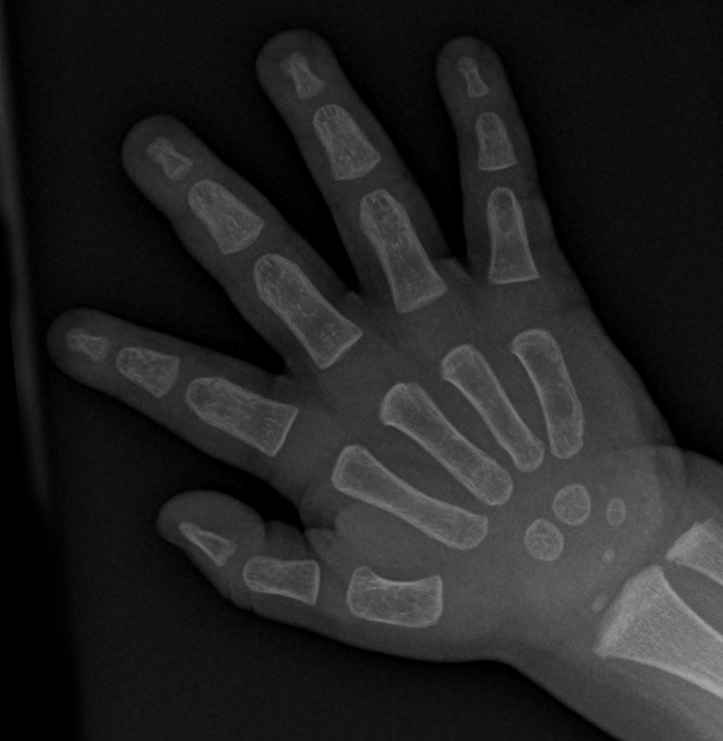
\includegraphics[width=.4\linewidth]{hand_1_1.png}}\hfill
 \subfloat[15 years old child.]{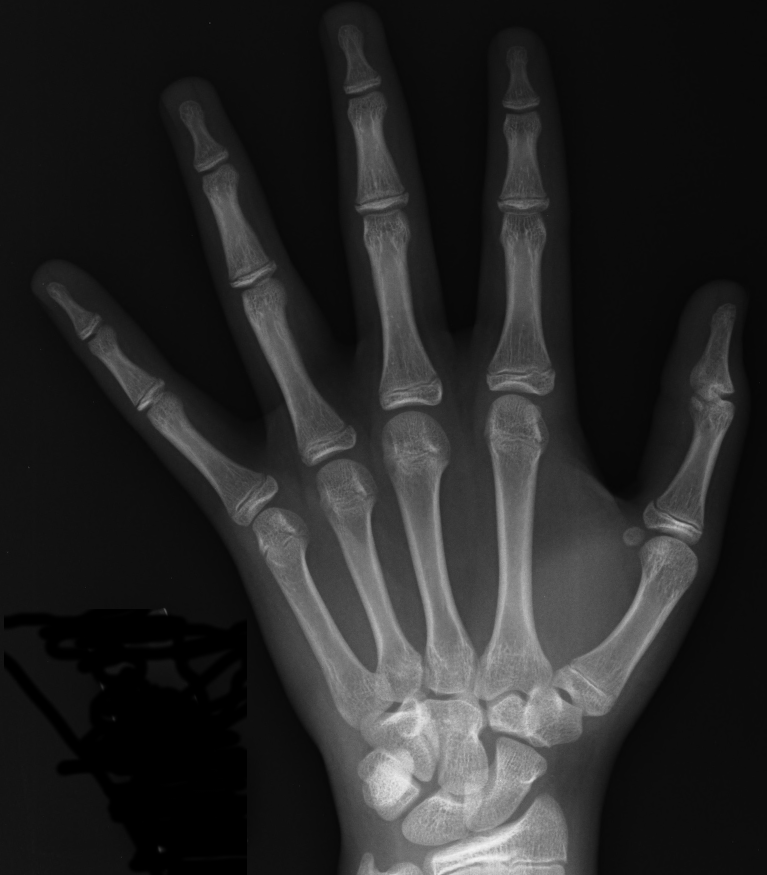
\includegraphics[width=.4\linewidth]{hand_15_1.png}}
 
 \caption{X-ray radiographies of hands. Copyright 2012 Mark Hammer and Guillermo Gonzalez. Images taken from \url{http://bones.getthediagnosis.org/}. }
 \label{fig:mispa:exam_2018:radio}
\end{figure}


\begin{qbox}
 Provide an automatic segmentation of the bones of the different images provided. You can manually avoid the annotations that may be present (most of them have been removed).
\end{qbox}
